%*============================================================*
%**Goal		:    文献分享:消失的女性与茶叶的价格
%**Author	:  	 ZhangYi zhangyiceee@163.com 15592606739
%**Created	:  	 20200323
%**Last Modified: 2020
%*============================================================*



\documentclass{beamer}
\usepackage[UTF8,noindent]{ctexcap}
\usepackage{natbib}
\usepackage{hyperref}
\usepackage{color}
\usepackage{natbib}

\graphicspath{{figures/}}




\usetheme{Madrid}
%\usecolortheme{crane} %黄色
%\usecolortheme{wolverine} %黄蓝
\usecolortheme{lily} %蓝白
%\usecolortheme{beetle} %灰色
%Information to be included in the title page:
\title[文献分享:ZY]{与祖辈同住:当前中国家庭的三代居住安排与青少年的学业表现}
\author[张帆、吴愈晓]{张帆、吴愈晓}
\date{\today}

\begin{document}

\frame{\titlepage}
%开始你的表演



%第1页幻灯片
%==========================================
\begin{frame}
\frametitle{Abstract}
通过分析具有全国代表性的初中学生样本数据,本研究考察了影响当前中国家庭三代共同居住的决定因素、三代居住安排与青少年学业表现之间的关系及其中间机制。首先,家庭社会经济地位较低、母亲在职或单亲家庭的青少年更可能与祖辈同住。其次,代际居住安排会显著影响青少年的学业表现,控制了其他因素之后,三代共同居住(与祖辈同住)家庭的学生的学 业表现要优于两代核心家庭的学生。 第三,与祖辈同住的效应受到家庭社会经济地位和家庭结构的调节,来自较低阶层或非双亲家庭的学生从与祖辈同住中获益更多。最后,与祖辈同住在一定程度上通过加强亲子间的家庭社会资本这一机制作用于学生的学业表现。本文表明,在现代社会,家庭亲属网络仍然对个体的地位获得或社会流动具有十分重要的作用。
\end{frame}

\begin{frame}
\frametitle{Problem}
% 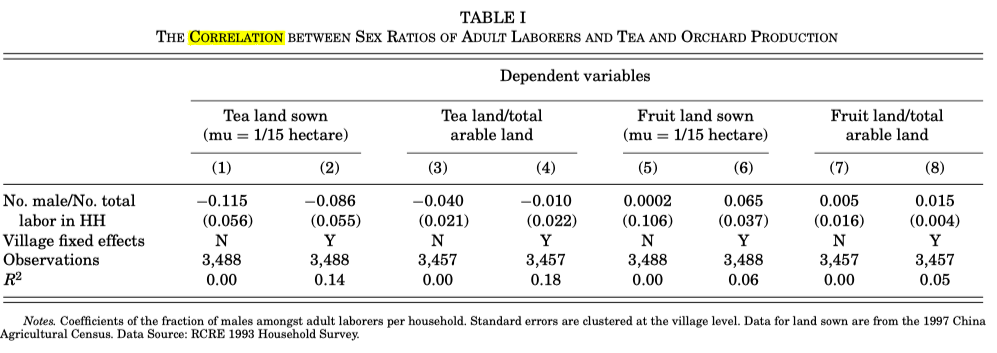
\includegraphics[scale=0.5]{table1}
祖辈对于孙辈的影响,以往研究都认为在控制了父辈因素之后,祖辈并不直接作用于孙辈的地位获取(马尔可夫过程)。
当前的研究中忽略了三代之间的居住安排模式。(非马尔可夫过程)

马尔可夫过程:某一时刻状态转移的概率只依赖于它的前一个状态。举个简单的例子,假如每天的天气是一个状态的话,那个今天是不是晴天只依赖于昨天的天气,而和前天的天气没有任何关系。

\end{frame}


\begin{frame}
\frametitle{Objective}
\begin{itemize}
	\item 与祖辈同住的影响因素	
	\item 与祖辈同住对学生学业表现的影响?
	\item 与祖辈同住如何通过社会资本的机制发挥作用?
\end{itemize}
\end{frame}


\begin{frame}
	\frametitle{理论分析:影响因素}
	费孝通的功能主义观点认为,家庭是一个由男女分工合作而形成的双系抚育的团体,它以抚育后代作为基本功能。现代社会,女性劳动参与率提高,因此需要调动上一代资源来缓解家庭的负担。
	\\ 一般而言家庭可以通过购买社会机构的服务来达到相同的目标。但是我国还未建立起完善的社会保障制度和家务劳动市场,而且家务市场是有钱人才请的起的。因此对于多数家庭来说,由祖辈照顾孙辈成为理性选择。---家庭社会经济地位越低,越有可能选择与父母同住
	\\ 父母缺位的家庭往往与较低的社会经济地位相关,且改革开放后离婚率上升、留守儿童出现。家庭双系抚育结构面临严重危机,因此作者推断:与双亲家庭相比,父母缺位家庭更加需要通过家庭网络来缓解由于父母缺位带来的家庭危机
\end{frame}

\begin{frame}
	\frametitle{与祖辈同住对学业表现的影响}
两种代表性观点:
	\begin{itemize}
		\item 祖辈与孙辈间的资源传递:祖辈拥有的声望、权力、社会地位以及经济财富会对后代产生庇护。即使祖辈离世这种效应仍然存在。
		\item 祖辈与孙辈间的互动:频繁的直接互动有助于提高祖辈对孙辈的各种资源传递的效率,进而对孙辈的地位获得和教育发展产生影响。
	\end{itemize}
根据以上两种观点,选择与祖辈同住都将有利于青少年的教育发展。
	异质性:与祖辈同住可能对低阶层家庭的孩子更为重要,孙辈从父辈可以获取的经济资源较少, 因此祖辈提供的经济资源就显得更有意义。
	\\ 与祖辈同住对于非双亲家庭的孩子的教育发展更为有利。
\end{frame}

\begin{frame}
	\frametitle{家庭社会资本--与祖辈同住的间接机制}
	从社会资本角度看,与两代核心家庭相比,祖辈的加入不仅会增加家庭的社会资本总量,更为重要的是,祖辈的存在可能会通过改善父辈与孙辈之间的社会资本间接地作用于孙辈的学业成就。家庭社会资本可分为(科尔曼,1988):
	\begin{itemize}
		\item 家庭内部社会资本:父母与子女间的有效互动,亲子间承诺、互惠和信任。
		\item 家庭外部社会资本:父母与社会内其他成员的社会关系以及父母与社会机构的联系。
	\end{itemize}
\end{frame}


\begin{frame}
	\frametitle{家庭社会资本--与祖辈同住的间接机制}
与祖辈同住如何影响家庭的社会资本?
\begin{itemize}
	\item 父辈和子辈同住扩展为三代同住,家庭社会资本由父子间+祖辈与父辈+祖辈与孙辈,家庭社会资本总量提升
	\item 现有分工体系下,祖辈承担更多的日常照料,那么父辈可以专注于孙辈的教育,进而有利于父辈与孙辈间社会资本质量的提高。
\end{itemize}
\end{frame}



\begin{frame}
	\frametitle{数据、变量与研究方法}
	\begin{itemize}
		\item 数据
		\item 变量
		\item 方法
	\end{itemize}
\end{frame}

\begin{frame}
	\frametitle{数据、变量与研究方法:数据}
	CEPS2014-2015年追踪数据,剔除掉了父母不在家的个案以及部分确实个案(确保可以测量亲子间的社会互动),得到样本总数8879个。
	\\ 后文关于与祖辈同住的定义中只要和祖辈同住就定义为1,其他为0,那么这里的样本会缺少很大一部分的隔代同住的家庭。
\end{frame}


\begin{frame}
	\frametitle{数据、变量与研究方法:变量}
	\begin{itemize}
		\item 学业表现:认知能力、考试成绩和自评学习能力(语数外学习困难程度的加总),主成分合成一个0-100的“学业表现变量”
		\item 是否与祖辈同住和家庭结构:“与祖辈同住”则赋值为1,根据学生与父母同住的情况将家庭结构分为:双亲、单亲父亲、单亲母亲家庭。
		\item 家庭社会经济地位
		\item 家庭社会资本
			\begin{itemize}
				\item 家庭内部社会资本:
					\begin{itemize}
						\item 亲子互动频率、父母的教育期望、学生的教育期望、亲子教育期望差异和父母对孩子未来的信心
					\end{itemize}
				\item 家庭外部的社会资本:
					\begin{itemize}
						\item 学生自身的社会资本:学校同辈群体质量、学生的集体融入和人际关系
						\item 家长社会资本:是否认识孩子朋友的父母、是否参加家长会、是否主动与老师联系
						
					\end{itemize}
			\end{itemize}
		\item 其他:性别、户口、流动儿童、兄弟姐妹数量等
	\end{itemize}
\end{frame}

\begin{frame}
	\frametitle{数据、变量与研究方法:方法}
	\begin{itemize}
		\item 区县随机效应Logit模型(考虑到区域间社会经济文化的差异)探究影响因素
		\item 学校固定效应模型:研究与祖辈同住对学业表现的影响及作用机制,为了克服选择行对估计结果的影响,采用稳定逆概率加权(IPTW)克服选择性对于估计结果产生的偏误。
	\end{itemize}
\end{frame}


\begin{frame}
\frametitle{Result:与祖辈同住的影响因素}
	\centering{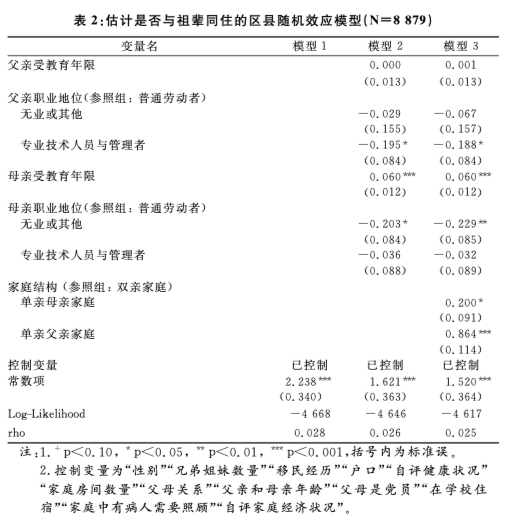
\includegraphics[scale=0.5]{table2}}
\end{frame}

\begin{frame}
\frametitle{Result:与祖辈同住的影响因素}
	模型2:在控制其他变量的情况下,母亲的受教育年限每增加一年,学生与祖辈同住几率比将增加约6\%($exp(0.060)-1 \approx 0.062,p<0.001$),同母亲为普通劳动者的学生相比,母亲为无业的学生与祖辈同住的几率要低18.4\%,母亲为专业技术人员和管理者的学生与祖辈同住几率比无差异。父亲的职业地位越高,学生越不可能与祖辈同住。
\\ 从家庭结构看,单亲家庭的学生与祖辈同住可能性更高,单亲母亲家庭的学生与祖辈同住分几率比要高22\%,单亲父亲家庭学生与祖辈同住几率比高达137\%,当母亲缺位时,家庭面临的儿童服与危机更为严重,与祖辈同住有助于缓解由于家庭机构被破坏而产生的压力,因此,单亲家庭的学生更容易与祖辈同住,特别是单亲父亲家庭。
\\ 表2检验了祖辈在现代家庭生活中的补充性角色。
\end{frame}

\begin{frame}
\frametitle{Result:与祖辈同住对青少年学业表现的群体异质性}	
	\centering{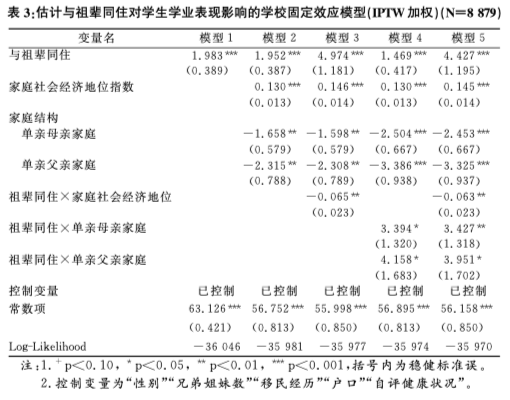
\includegraphics[scale=0.5]{table3}}
	\\ 与祖辈同住会提高青少年的学业表现
\end{frame}

\begin{frame}
\frametitle{Result:与祖辈同住对青少年学业表现的群体异质性}	
	\centering{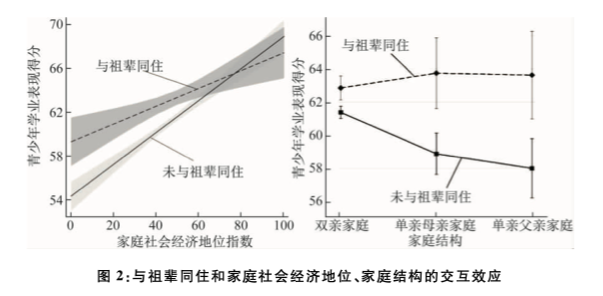
\includegraphics[scale=0.5]{figure2}}
\end{frame}

\begin{frame}
	\frametitle{对于学业表现影响的异质性}
主要考察与祖辈同住对来自不同家庭社会经济地位和家庭结构的青少年的异质性影响。
\begin{itemize}
	\item 与不同住的青少年相比,同住的青少年的家庭社会经济地位每增加一个单位,同住的效应降低0.065
	\item 与祖辈同住对于单亲家庭的孩子有明显的补偿作用,
\end{itemize}
\end{frame}


\begin{frame}
	\frametitle{Result:间接机制---家庭社会资本}
	\centering{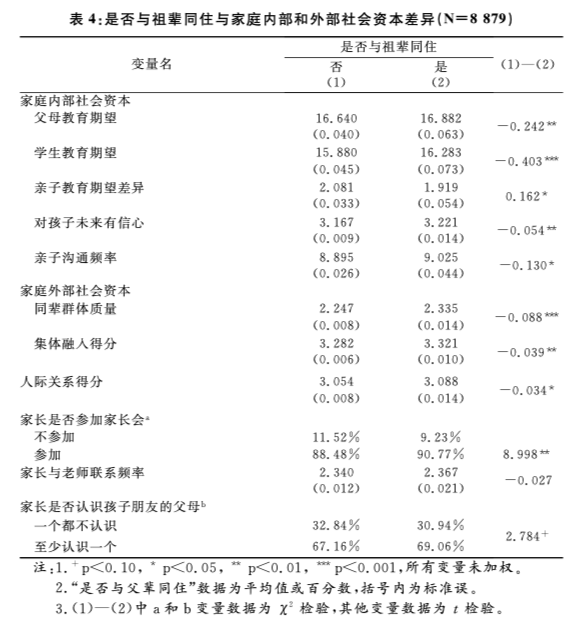
\includegraphics[scale=0.4]{table4}}

\end{frame}


\begin{frame}
	\frametitle{Result:间接机制---家庭社会资本}
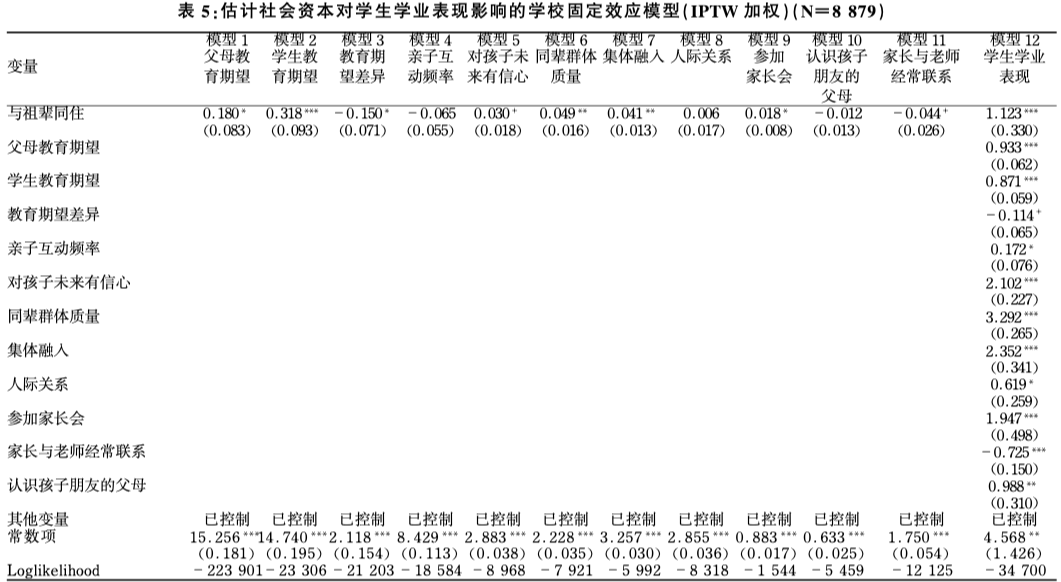
\includegraphics[scale=0.32]{table5}
\end{frame}

\begin{frame}
	\frametitle{吴愈晓\&感想}
 吴愈晓:为什么教育竞争愈演愈烈?串联了他自己的很多研究,其中就包括三代同住 \url{https://www.bilibili.com/video/BV1p5411W78i?from=search&seid=16354117810740553962}

 \begin{itemize}
		\item 社会学与经济学的不同,尤其在写作上;
		\item 与中国工业经济类似,“社会”提供早期(最近一期是2019年)文章的dofile,可以复制学习。\url{http://www.society.shu.edu.cn/CN/item/showItemList.do?pager=1&columnId=40}
\end{itemize}

\end{frame}


\begin{frame}
	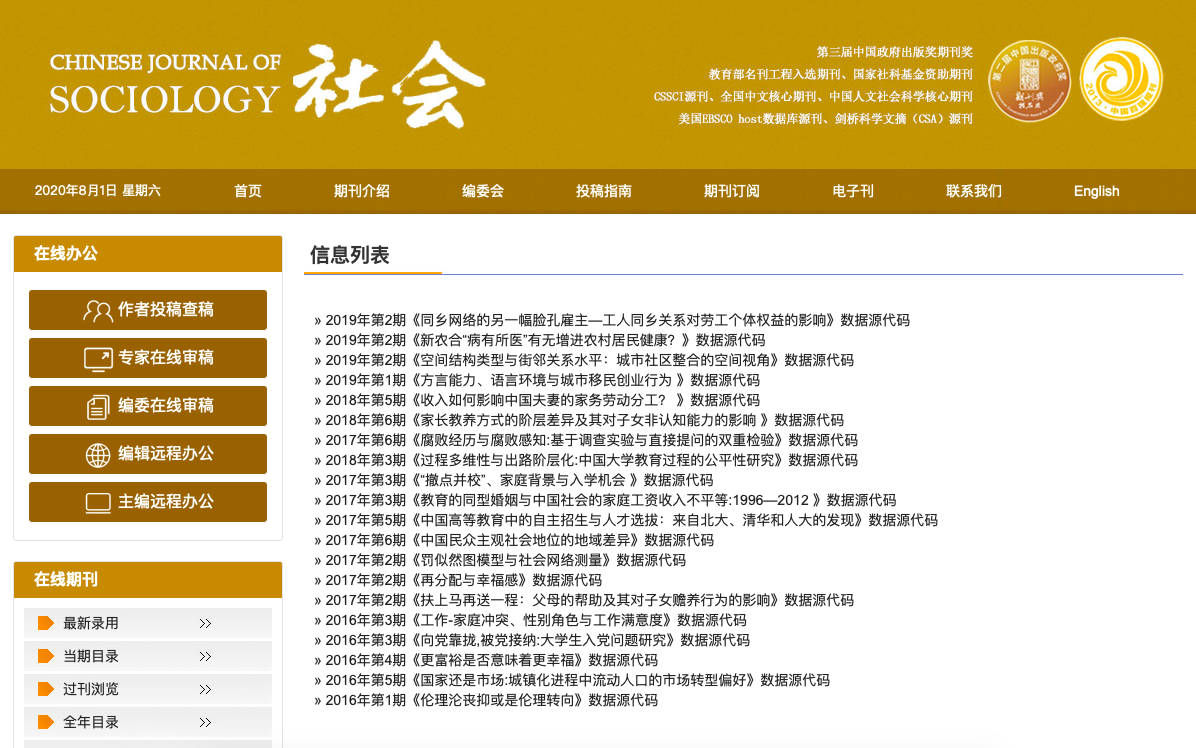
\includegraphics[scale=0.3]{社会}
\end{frame}
%参考文献的案例 \citet{Krueger1999Experimental} \citep{Krueger1999Experimental}  注意两类的不同
\end{document}



